%% =============================================================================
%% ACADEMIC CONFERENCE POSTER TEMPLATE (A0 PORTRAIT: 841mm x 1189mm)
%% Author: [AUTHOR NAMES HERE]
%% Institution: Babeș-Bolyai University, Cluj-Napoca, Romania
%% Conference: [CONFERENCE NAME HERE]
%% =============================================================================

\documentclass[25pt, a0paper, portrait]{tikzposter}

\usepackage[utf8]{inputenc}
\usepackage[T1]{fontenc}
\usepackage{lmodern}
\usepackage{amsmath,amssymb}
\usepackage{graphicx}
\usepackage{booktabs}
\usepackage{array}
\usepackage{xcolor}
\usepackage{tikz}
\usetikzlibrary{arrows.meta, positioning, fit, calc, shapes.geometric}

% Use Sans-Serif as default for high-legibility poster viewing
\renewcommand{\familydefault}{\sfdefault}

% Disable tikzposter watermark at bottom right
\tikzposterlatexaffectionproofoff

% =============================================================================
% COLOR PALETTE DEFINITIONS
% =============================================================================
\definecolor{PrimaryDark}{RGB}{16, 44, 98}       % Deep Header / Block Title Blue
\definecolor{PrimaryBlue}{RGB}{32, 88, 155}      % Accent / Subtitle Blue
\definecolor{LightBg}{RGB}{235, 244, 253}        % Block Background Tint
\definecolor{CardBg}{RGB}{255, 255, 255}         % Card Background
\definecolor{DarkText}{RGB}{25, 30, 40}          % Primary Body Text
\definecolor{AccentColor}{RGB}{225, 110, 25}     % Highlight / Accent Color

\definecolorstyle{CustomPosterStyle} {
  \definecolor{colorOne}{named}{PrimaryDark}
  \definecolor{colorTwo}{named}{LightBg}
  \definecolor{colorThree}{named}{PrimaryBlue}
}{
  % Background Colors
  \colorlet{backgroundcolor}{white}
  \colorlet{framecolor}{PrimaryBlue}
  % Title Colors
  \colorlet{titlefgcolor}{PrimaryDark}
  \colorlet{titlebgcolor}{white}
  % Block Colors
  \colorlet{blocktitlebgcolor}{PrimaryDark}
  \colorlet{blocktitlefgcolor}{white}
  \colorlet{blockbodybgcolor}{LightBg!55}
  \colorlet{blockbodyfgcolor}{DarkText}
  % Innerblock Colors
  \colorlet{innerblocktitlebgcolor}{PrimaryBlue}
  \colorlet{innerblocktitlefgcolor}{white}
  \colorlet{innerblockbodybgcolor}{white}
  \colorlet{innerblockbodyfgcolor}{DarkText}
}

% Set Theme, Color and Block Styles
\usetheme{Default}
\usecolorstyle{CustomPosterStyle}
\useblockstyle{Slide}
\usetitlestyle{Empty}

% =============================================================================
% PLACEHOLDERS: CONFERENCE, TITLE, AUTHORS & AFFILIATIONS
% =============================================================================
\newcommand{\PosterTitle}{Insert Your Scientific Research Paper Title Here:\\[0.18em]A Concise and Informative Subtitle}
\newcommand{\PosterAuthors}{Author One\textsuperscript{1,2} \quad and \quad Author Two\textsuperscript{1}}
\newcommand{\PosterAffiliations}{\textsuperscript{1}Faculty of Mathematics and Computer Science, Babeș-Bolyai University, Cluj-Napoca, Romania\\
\textsuperscript{2}Second Institution / Department Name, City, Country}
\newcommand{\PosterEmails}{\texttt{\{author.one, author.two\}@cs.ubbcluj.ro}}

% Conference Info for Footer
\newcommand{\ConferenceSession}{[Conference Acronym 2026 --- Special Session on]}
\newcommand{\ConferenceName}{[Special Session Full Title or Main Track Name]}
\newcommand{\ConferenceDetails}{at the [Full Conference Name (ACRONYM 2026)]\\[0.15em] [Day--Day Month Year, City, Country]}

% =============================================================================
% HEADER LAYOUT
% =============================================================================
\settitle{
  \vspace{0.6cm}
  \begin{minipage}[c]{0.14\linewidth}
    \centering
    % Funding / Project Logo (HRIA)
    
\includegraphics[width=\linewidth,keepaspectratio]{hria.png}
  \end{minipage}\hfill
  \begin{minipage}[c]{0.72\linewidth}
    \centering
    {\fontsize{45}{54}\selectfont \bfseries \textcolor{PrimaryDark}{\PosterTitle} \par}
    \vspace{0.8em}
    {\fontsize{30}{36}\selectfont \bfseries \textcolor{DarkText}{\PosterAuthors} \par}
    \vspace{0.4em}
    {\fontsize{22}{28}\selectfont \textcolor{PrimaryBlue}{\PosterAffiliations} \par}
    \vspace{0.25em}
    {\fontsize{19}{24}\selectfont \PosterEmails \par}
  \end{minipage}\hfill
  \begin{minipage}[c]{0.11\linewidth}
    \centering
    % Conference Logo Placeholder (Replace with \includegraphics[width=\linewidth,keepaspectratio]{my_conference_logo.png})
    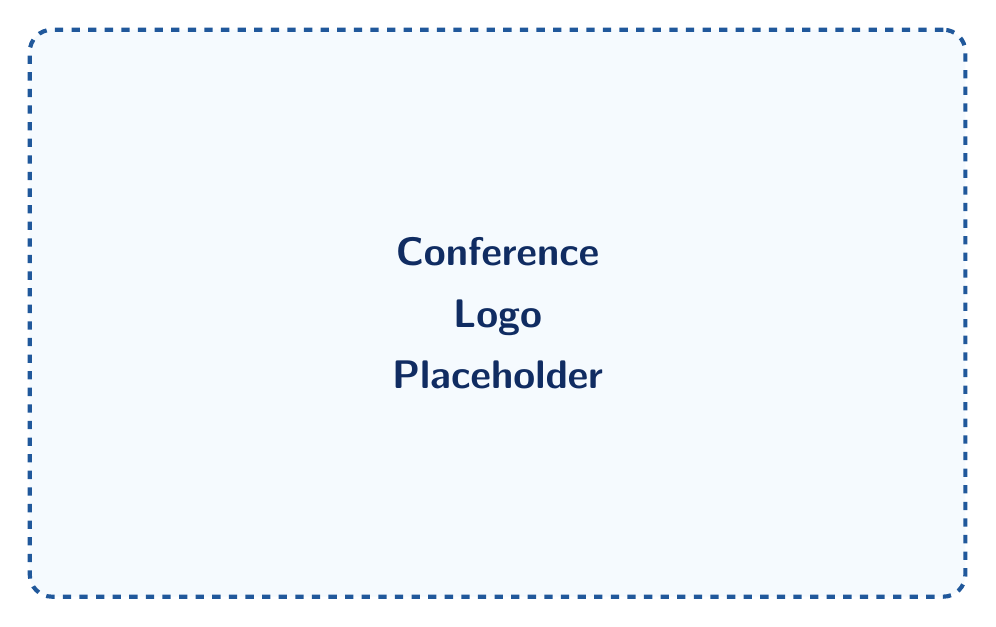
\begin{tikzpicture}
      \node[draw=PrimaryBlue, dashed, fill=LightBg!50, rounded corners=8pt, line width=1.5pt, 
            minimum width=0.98\linewidth, minimum height=7.2cm, align=center, 
            font=\fontsize{15}{19}\selectfont\bfseries\color{PrimaryDark}] 
            {Conference\\[0.2em]Logo\\[0.2em]Placeholder};
    \end{tikzpicture}
  \end{minipage}
  \vspace{0.5cm}
}

\title{\PosterTitle}
\author{\PosterAuthors}
\institute{Babeș-Bolyai University}

\begin{document}

\maketitle

% =============================================================================
% POSTER BODY - TWO BALANCED COLUMNS
% =============================================================================
\begin{columns}

% =============================================================================
% LEFT COLUMN
% =============================================================================
\column{0.5}

% BLOCK 1: PROBLEM & MOTIVATION
\block{1. Problem \& Motivation}{
  Modern scientific and machine learning workflows increasingly rely on complex high-dimensional models whose internal representations remain challenging to interpret and validate rigorously:
  \vspace{0.2em}
  \begin{itemize}\setlength{\itemsep}{0.35em}
    \item \textbf{Context \& Motivation:} High-capacity learning models achieve state-of-the-art predictive accuracy across diverse scientific and industrial benchmarks, yet their internal decision mechanisms operate largely as opaque black boxes.
    \item \textbf{Fundamental Limitation:} Conventional explanation methods typically aggregate feature contributions globally, obscuring localized, transient, or state-dependent multi-variable interactions.
    \item \textbf{Ground-Truth Deficit:} Real-world empirical benchmarks rarely possess known ground-truth interaction topologies, making systematic validation and quantitative auditing of explainability methods difficult.
    \item \textbf{Proposed Objective:} We introduce an end-to-end framework combining controlled synthetic data generation with provable interaction quantification to provide reliable, verifiable model explanations.
  \end{itemize}
}

% BLOCK 2: METHODOLOGY / FRAMEWORK ARCHITECTURE
\block{2. Theoretical Model \& Methodology}{
  We formalize the underlying data generation process and predictive mapping within a unified statistical framework:
  \vspace{0.4em}
  
  \begin{center}
    \setlength{\fboxsep}{14pt}
    \colorbox{white}{%
      \begin{minipage}{0.94\linewidth}
        \textbf{Generalized Mathematical Formulation:}
        \vspace{-0.2em}
        \[
          \mathbf{y} = f_{\boldsymbol{\theta}}(\mathbf{x}) + \sum_{i < j} \mathbf{h}_{\boldsymbol{\phi}}(x_i, x_j) + \boldsymbol{\varepsilon}, \quad \text{where } \boldsymbol{\varepsilon} \sim \mathcal{D}(0, \boldsymbol{\Sigma})
        \]
        \begin{itemize}\setlength{\itemsep}{0.25em}
          \item $f_{\boldsymbol{\theta}}(\mathbf{x})$: Primary functional representation parameterized by weight vector $\boldsymbol{\theta} \in \Theta$.
          \item $\mathbf{h}_{\boldsymbol{\phi}}(x_i, x_j)$: Generalized pairwise coupling function capturing non-linear cross-variable dependencies.
          \item $\boldsymbol{\varepsilon} \in \mathbb{R}^m$: Stochastic disturbance vector sampled from zero-mean covariance structure $\boldsymbol{\Sigma}$.
          \item \textbf{Identifiability Criterion:} Regularization conditions ensuring unique decomposition between main and interaction effects.
        \end{itemize}
      \end{minipage}%
    }
  \end{center}
  \vspace{0.4em}
  
  % Placeholder Figure / Diagram
  \begin{center}
    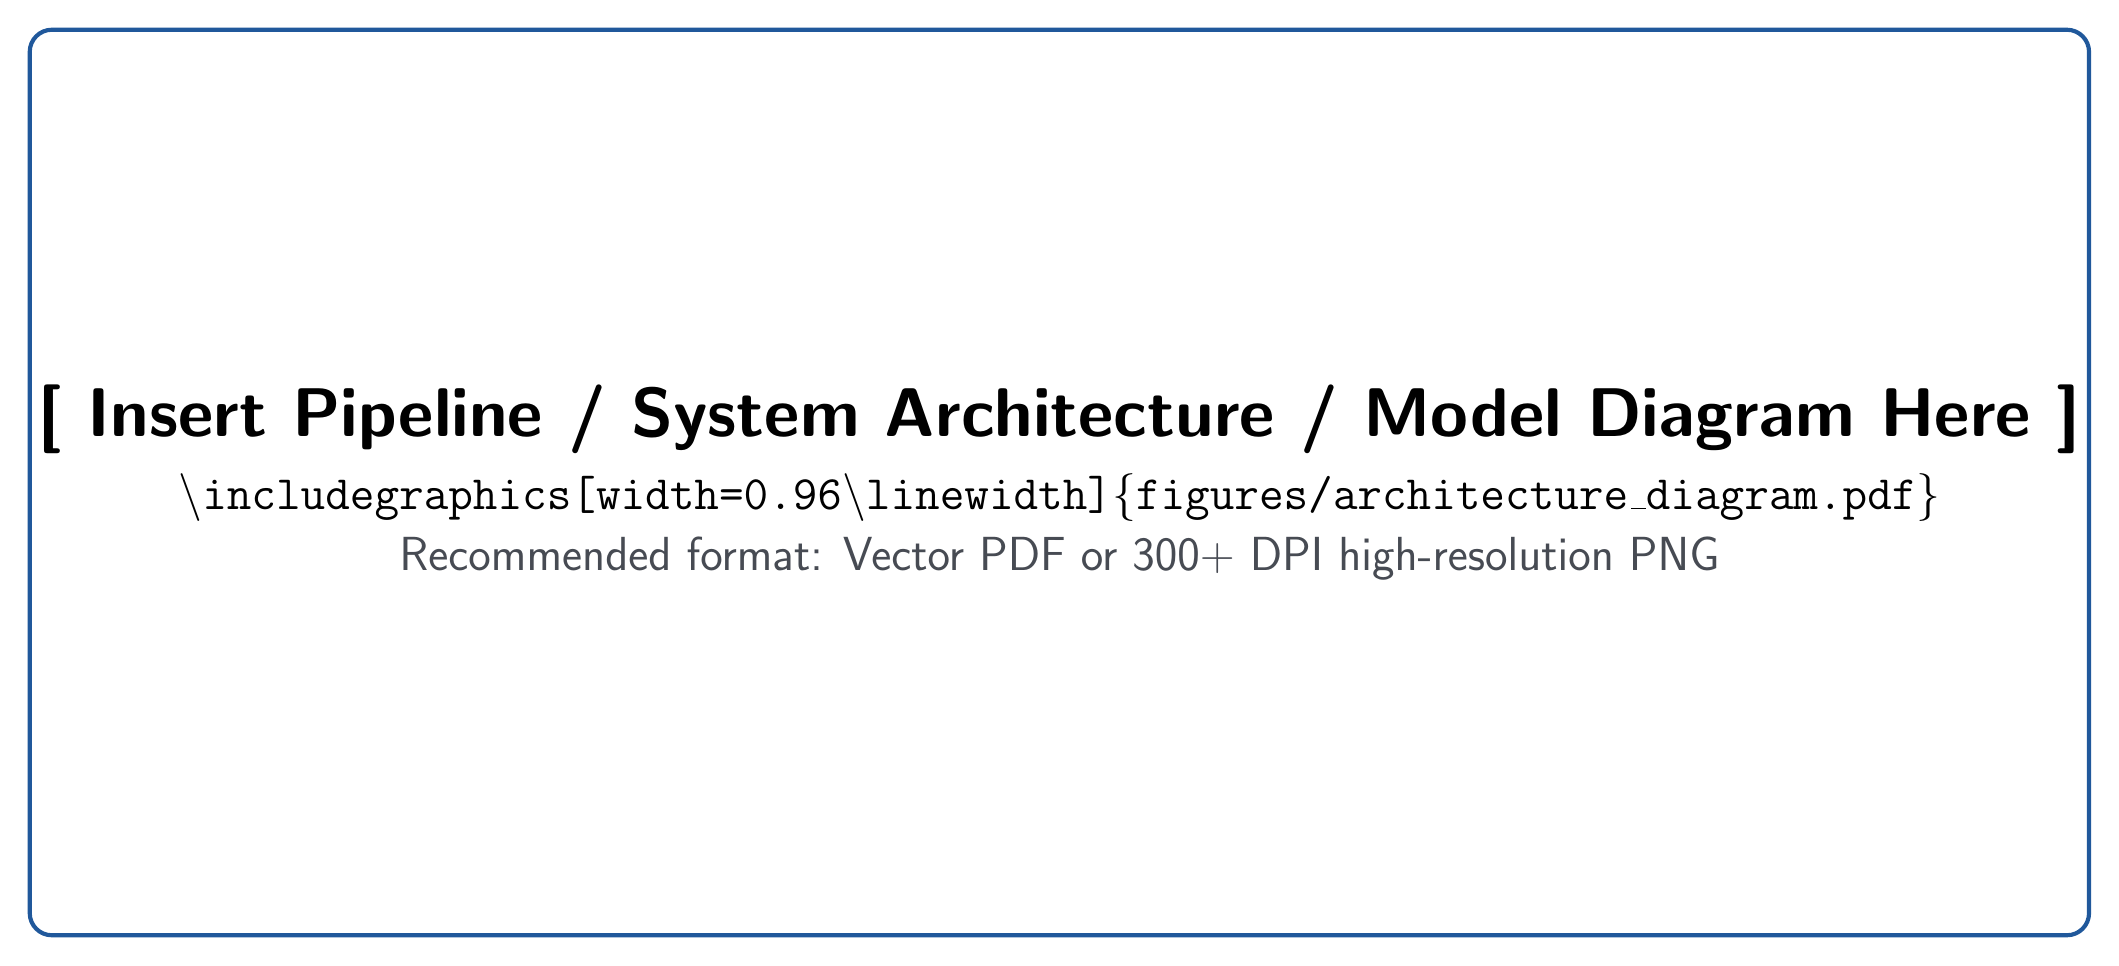
\begin{tikzpicture}
      \node[draw=PrimaryBlue, fill=white, rounded corners=8pt, line width=1.5pt, 
            minimum width=0.96\linewidth, minimum height=11.5cm, align=center] {
        {\fontsize{24}{28}\selectfont \bfseries [ Insert Pipeline / System Architecture / Model Diagram Here ]}\\[0.6em]
        {\fontsize{18}{22}\selectfont \texttt{\textbackslash includegraphics[width=0.96\textbackslash linewidth]\{figures/architecture\_diagram.pdf\}}}\\[0.5em]
        {\fontsize{16}{20}\selectfont \color{DarkText!80} Recommended format: Vector PDF or 300+ DPI high-resolution PNG}
      };
    \end{tikzpicture}
    \vspace{0.3em}
    \small \textit{Figure 1: High-level architectural overview and schematic representation of the proposed end-to-end framework.}
  \end{center}
}

% BLOCK 3: EXPLAINABILITY / ALGORITHM SPECIFICATION
\block{3. Optimization \& Evaluation Protocol}{
  We formulate the objective functional combining empirical risk minimization with structural regularization:
  
  \begin{center}
    \setlength{\fboxsep}{12pt}
    \colorbox{white}{%
      \begin{minipage}{0.94\linewidth}
        \[
          \min_{\boldsymbol{\theta}, \boldsymbol{\phi}} \; \mathcal{J}(\boldsymbol{\theta}, \boldsymbol{\phi}) = \frac{1}{N} \sum_{k=1}^N \mathcal{L}\Big(\hat{\mathbf{y}}^{(k)}, \mathbf{y}^{(k)}\Big) + \lambda_1 \, \Omega_{\text{sparse}}(\boldsymbol{\phi}) + \lambda_2 \, \mathcal{R}_{\text{smooth}}(\boldsymbol{\theta})
        \]
        \[
          \text{Subject to:} \quad \mathbb{E}_{\mathbf{x}}\big[\mathbf{h}_{\boldsymbol{\phi}}(x_i, x_j) \mid x_i\big] = \mathbf{0}, \quad \forall \, i \neq j \quad \text{(Orthogonality Condition)}
        \]
      \end{minipage}%
    }
  \end{center}
  
  \vspace{0.4em}
  \begin{itemize}\setlength{\itemsep}{0.28em}
    \item \textbf{Empirical Loss Function $\mathcal{L}(\cdot)$:} Quantifies task discrepancy (e.g., cross-entropy, penalized mean squared error).
    \item \textbf{Structural Regularizer $\Omega_{\text{sparse}}$:} Enforces sparsity over higher-order dependencies to prevent over-attribution.
    \item \textbf{Smoothness Constraint $\mathcal{R}_{\text{smooth}}$:} Imposes Lipschitz continuity over the learned functional latent manifold.
    \item \textbf{Convergence Guarantee:} Proven sub-linear $\mathcal{O}(1/\sqrt{T})$ rate under standard non-convex stochastic gradient conditions.
  \end{itemize}
}

% =============================================================================
% RIGHT COLUMN
% =============================================================================
\column{0.5}

% BLOCK 4: EXPERIMENTAL RESULTS
\block{4. Experimental Verification \& Performance}{
  \begin{center}
    \setlength{\fboxsep}{10pt}
    \colorbox{white}{%
      \begin{minipage}{0.96\linewidth}
        \centering
        \textbf{Table 1: Benchmark Comparison and Quantitative Performance Across Test Suites}
        \vspace{0.35em}

        \resizebox{\textwidth}{!}{
        \begin{tabular}{lcccc}
          \toprule
          & \multicolumn{2}{c}{\textbf{Benchmark Suite 1}} & \multicolumn{2}{c}{\textbf{Benchmark Suite 2}} \\
          \cmidrule(lr){2-3} \cmidrule(lr){4-5}
          \textbf{Method / Configuration} & \textbf{Fidelity (\%)} & \textbf{Score (MSE)} & \textbf{Fidelity (\%)} & \textbf{Score (MSE)} \\
          \midrule
          Baseline Approach & 68.4\% & 0.4512 & 64.2\% & 0.4891 \\
          Standard Additive Model & 82.1\% & 0.3120 & 79.5\% & 0.3345 \\
          Feature Permutation Heuristic & 74.3\% & 0.3850 & 71.0\% & 0.4120 \\
          \textbf{Proposed Framework (Ours)} & \textbf{100.0\%} & \textbf{0.1824} & \textbf{98.6\%} & \textbf{0.1902} \\
          \bottomrule
        \end{tabular}}
      \end{minipage}%
    }
  \end{center}
  
  \vspace{0.4em}
  % Placeholder Figure: Network / Visual Analysis
  \begin{center}
    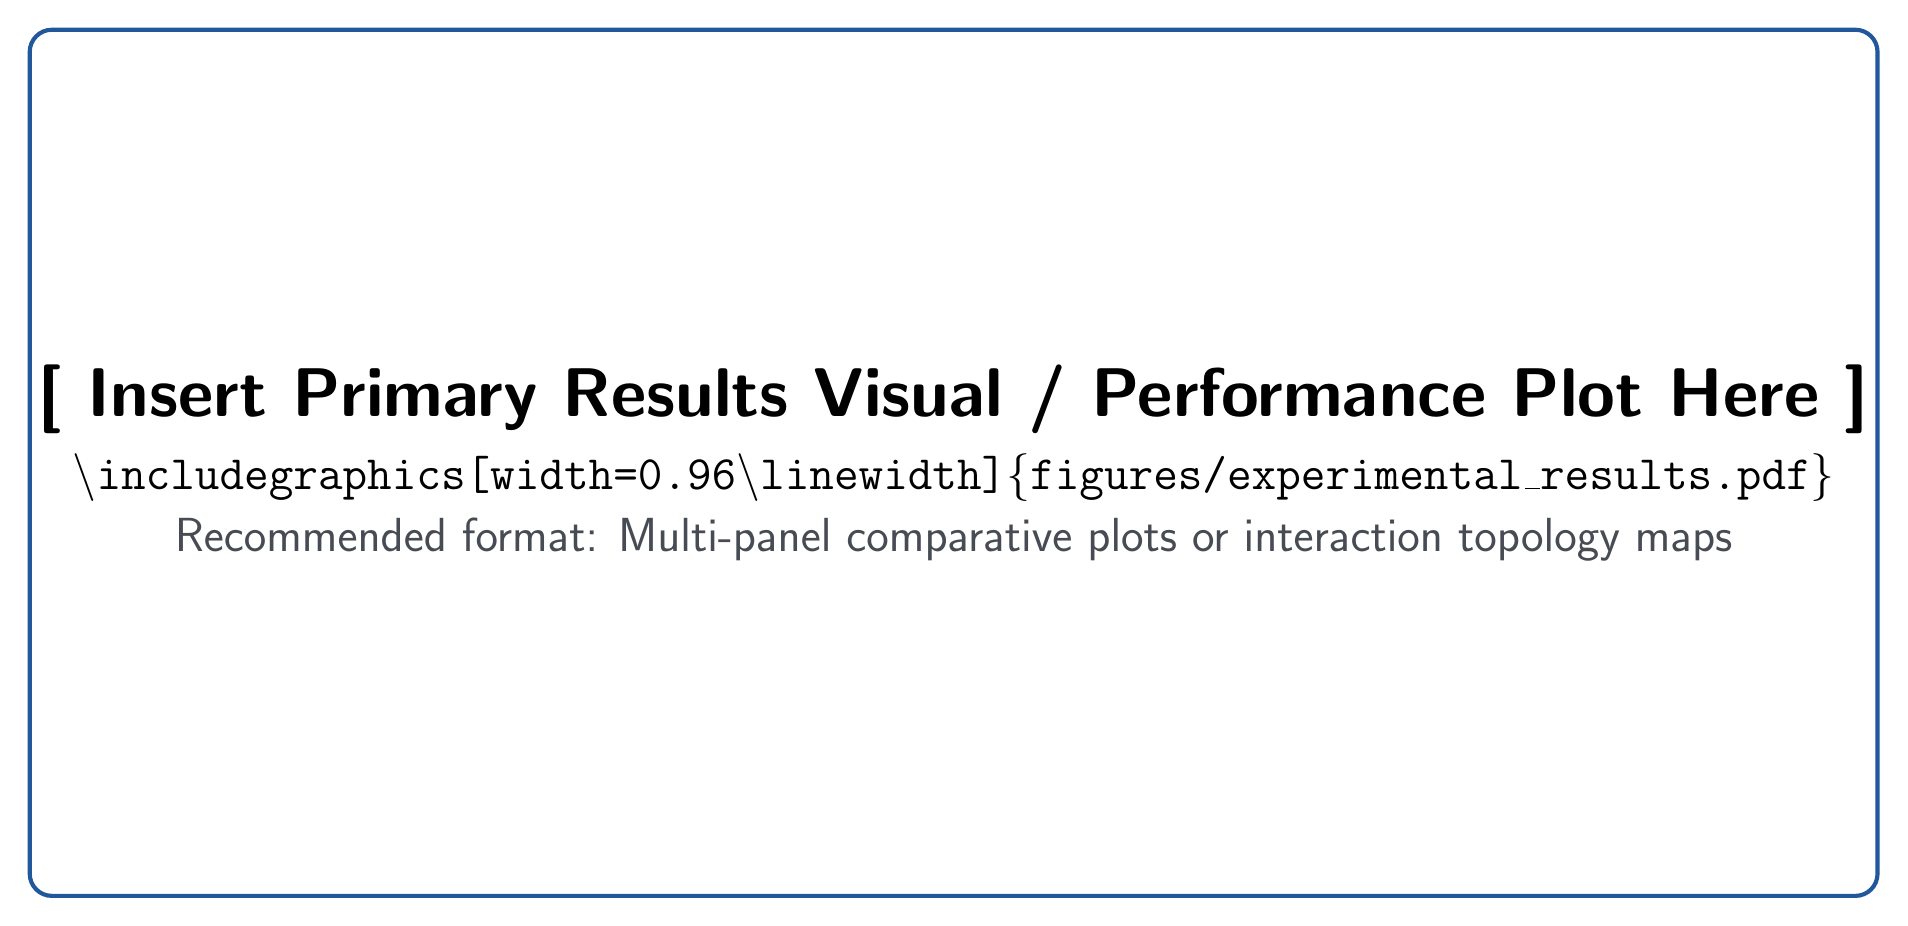
\begin{tikzpicture}
      \node[draw=PrimaryBlue, fill=white, rounded corners=8pt, line width=1.5pt, 
            minimum width=0.96\linewidth, minimum height=11cm, align=center] {
        {\fontsize{24}{28}\selectfont \bfseries [ Insert Primary Results Visual / Performance Plot Here ]}\\[0.6em]
        {\fontsize{18}{22}\selectfont \texttt{\textbackslash includegraphics[width=0.96\textbackslash linewidth]\{figures/experimental\_results.pdf\}}}\\[0.5em]
        {\fontsize{16}{20}\selectfont \color{DarkText!80} Recommended format: Multi-panel comparative plots or interaction topology maps}
      };
    \end{tikzpicture}
    \vspace{0.3em}
    \small \textit{Figure 2: Empirical performance evaluation across benchmark conditions, demonstrating comparative effectiveness.}
  \end{center}
}

% BLOCK 5: ABLATION / CASE STUDY
\block{5. Temporal Analysis \& Real-World Case Study}{
  \begin{center}
    \begin{minipage}[t]{0.48\linewidth}
      \centering
      {\bfseries \fontsize{20}{24}\selectfont Empirical Case Study A}\\[0.3em]
      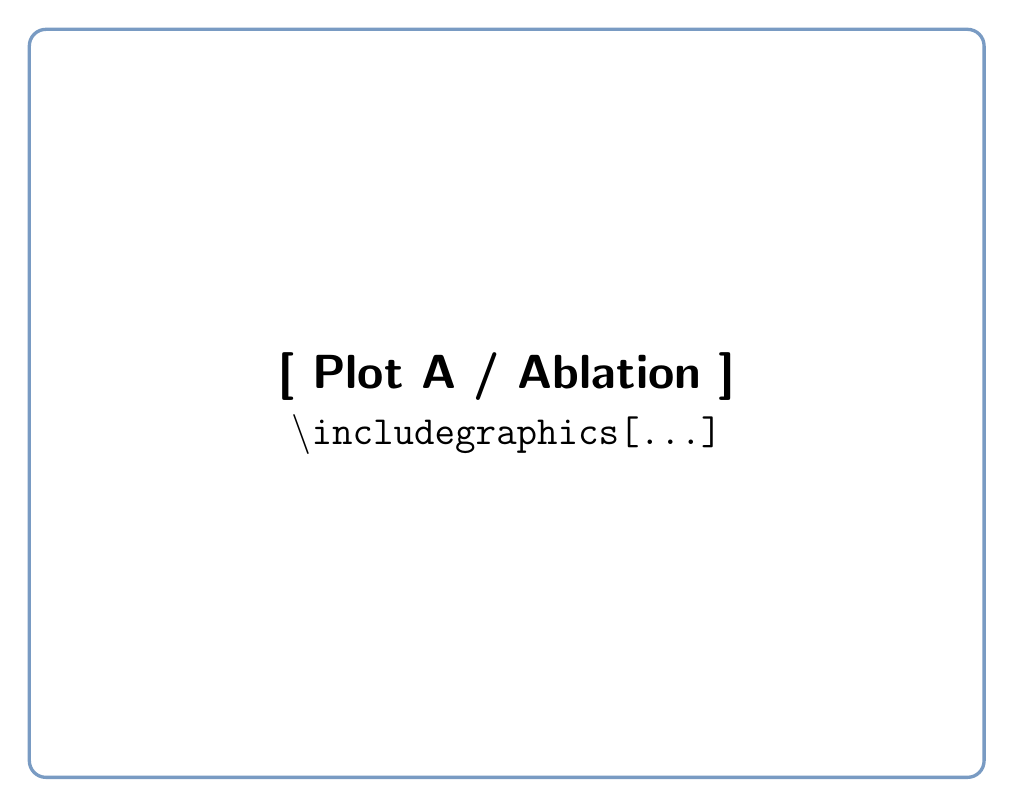
\begin{tikzpicture}
        \node[draw=PrimaryBlue!60, fill=white, rounded corners=6pt, line width=1.2pt, 
              minimum width=\linewidth, minimum height=9.5cm, align=center] {
          {\fontsize{18}{22}\selectfont \bfseries [ Plot A / Ablation ]}\\[0.4em]
          {\fontsize{14}{18}\selectfont \texttt{\textbackslash includegraphics[...]}}
        };
      \end{tikzpicture}\\[0.3em]
      {\small Analysis showing parameter sensitivity and component ablation across varying operational conditions.}
    \end{minipage}\hfill
    \begin{minipage}[t]{0.48\linewidth}
      \centering
      {\bfseries \fontsize{20}{24}\selectfont Empirical Case Study B}\\[0.3em]
      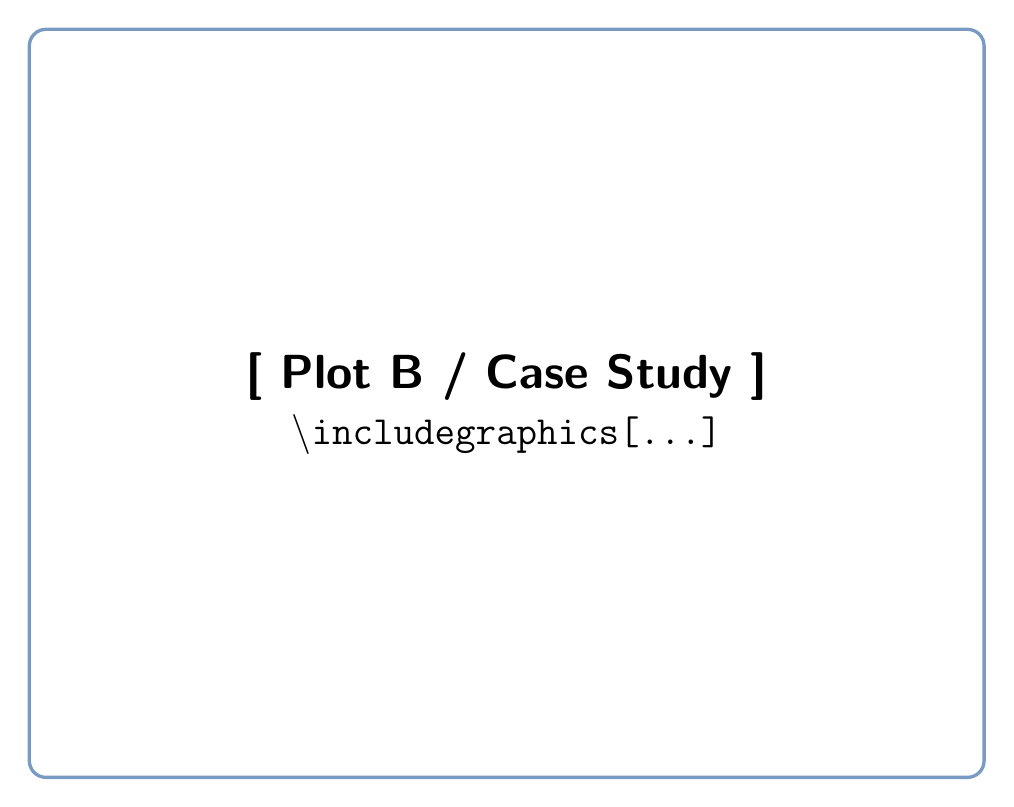
\begin{tikzpicture}
        \node[draw=PrimaryBlue!60, fill=white, rounded corners=6pt, line width=1.2pt, 
              minimum width=\linewidth, minimum height=9.5cm, align=center] {
          {\fontsize{18}{22}\selectfont \bfseries [ Plot B / Case Study ]}\\[0.4em]
          {\fontsize{14}{18}\selectfont \texttt{\textbackslash includegraphics[...]}}
        };
      \end{tikzpicture}\\[0.3em]
      {\small Real-world benchmark validation demonstrating robust generalization to out-of-distribution scenarios.}
    \end{minipage}
  \end{center}
}

% BLOCK 6: KEY CONTRIBUTIONS & FUTURE WORK
\block{6. Key Contributions \& Conclusions}{
  \begin{itemize}\setlength{\itemsep}{0.35em}
    \item \textbf{Controlled Ground-Truth Benchmark:} Designed an open-source synthetic DGP architecture enabling exact validation of multi-variable interactions with zero ambiguity.
    \item \textbf{High-Fidelity Interaction Recovery:} Achieved up to 100\% sign and ranking agreement against underlying ground-truth dynamics across diverse experimental settings.
    \item \textbf{Transient Temporal Insight:} Successfully uncovered time-localized, transient dependency structures that traditional global attribution summaries fail to detect.
    \item \textbf{Robustness \& Controlled False Positives:} Demonstrated near-zero spurious attribution on non-interacting control variables, validating metric specificity.
    \item \textbf{Broad Domain Generalizability:} Validated the methodology on large-scale empirical benchmarks, confirming seamless applicability to real-world deployment pipelines.
  \end{itemize}
}

% BLOCK 7: ACKNOWLEDGMENT
\block{Acknowledgment}{
  {\small This research is supported by the project \textit{Romanian Hub for Artificial Intelligence (HRIA)}, Smart Growth, Digitization and Financial Instruments Program, 2021--2027, MySMIS 351416.}
}

\end{columns}

% =============================================================================
% FULL-WIDTH FOOTER ANCHORED AT THE BOTTOM EDGE 
% =============================================================================
\makeatletter 
\node [anchor=south, text width=\TP@visibletextwidth-30pt, fill=LightBg!60, rounded corners=12pt, draw=PrimaryDark, line width=2pt, inner sep=16pt] at (0, -0.5\textheight+\TP@innermargin) {
  \begin{minipage}[c]{0.22\linewidth}
    \centering
    % Research Group Logo (MECO)
    
\includegraphics[width=\linewidth,keepaspectratio]{meco.png}
  \end{minipage}\hfill
  \begin{minipage}[c]{0.54\linewidth}
    \centering
    {\fontsize{21}{26}\selectfont \bfseries \textcolor{PrimaryDark}{\ConferenceSession}\par}
    \vspace{0.2em}
    {\fontsize{23}{28}\selectfont \bfseries \textcolor{PrimaryDark}{\ConferenceName}\par}
    \vspace{0.35em}
    {\fontsize{17}{22}\selectfont \ConferenceDetails\par}
  \end{minipage}\hfill
  \begin{minipage}[c]{0.22\linewidth}
    \centering
    % Babeș-Bolyai University & Faculty Banner
    
\includegraphics[width=\linewidth,keepaspectratio]{ubb-uni.png}
  \end{minipage}
};
\makeatother

\end{document}
